\newcommand\blfootnote[1]{%
  \begingroup
  \renewcommand\thefootnote{}\footnote{#1}%
  \addtocounter{footnote}{-1}%
  \endgroup
}

\chapter{INTRODUCTION}
\label{chapter:introduction}
\section{Particle physics experiments}
\blfootnote{This work was supported by the National Commission for Scientific and Technological Research (CONICYT) of Chile, under grant FONDECYT 11110165 and scholarship CONICYT-PCHA/Mag\'ister Nacional/2013 - folio 221320673.} Particle physics, also called High Energy Physics, is the branch of physics that studies the fundamental constituents of matter and radiation, and their mutual interactions. It aims to answer some of the profound questions of physics, with benefits spanning everything from advancing humankind’s understanding of the universe, to applications in other fields of science as well as daily life \citep{tuttle101}.

The main tools used by experimental particle physicists are particle accelerators, which use electromagnetic fields to accelerate charged particles to relativistic speeds before they are made to collide inside detectors. The detectors gather clues about the particles – including their speed, mass and charge – from which physicists can work out a particle's identity \citep{cern101}. An example of such an accelerators is the Large Hadron Collider (LHC) at \emph{Organisation européenne pour la recherche nucléaire} (CERN), which recently proved the existence of the Higgs field \citep{Aad:2012tfa, Chatrchyan:2012ufa}, a key element to complete the Standard Model and one of the greatest scientific achievements of the past 50 years. 
%fantastic triumph for Science \citep{nobel}.

Because experimenters seek ever-increasing high-energy collisions to make new discoveries, and because there are greatest discoveries yet to be made, new and larger particle accelerators appear in the roadmap of the scientific community. Up to date, there are two projects in the race to define the LHC's successor, the International Linear Collider (ILC) and the Compact Linear Collider (CLIC), both coordinated by the Linear Collider Collaboration. 

As the collision energy increases with each new accelerator generation, so does the complexity of the detectors used to gather information about the collisions. This makes it necessary a continuous improvement of the techniques used in instrumentation for particle physics. An example of this is the introduction of the CMOS technology in the early 80's, which changed the trend of detector front-end electronics from printed circuit boards (PCBs) to custom integrated circuits, improving integration and allowing on-site electronics with a minimum of mass added to the detector system \citep{abuslemethesis}. 

This thesis deals with an emerging trend to improve the electronics used in particle physics: the use of discrete-time filters to lower the noise present in the detectors front-end circuits. A new mathematical framework for noise analysis of discrete-time filters is presented, in an attempt to guide a proper filter design when a discrete-time filter is used for pulse-processing purposes. Additionally, the design and characterization of a front-end filter for one of the detectors planned for the ILC is presented.


%The current trends are to include more channels, increased processing capabilities, lower noise, and better radiation hardness, all within the power budget available \citep{abuslemethesis}. 


%The purpose of this paper is twofold.

%This thesis deals with an emerging trend in electronics for particle physics, the use of discrete-time filters to lower the noise present in a detectors front-end circuit.

 
%This thesis deals with one of this trends, achieve low noise electronics by means of the use of discrete-time filters

%low noise circuits, in particular the design of a framework to systematize the design of discrete-time filters used in instrumentation for particle physics.

% These beams are used to generate particle collisions, either by means of the impact of one of them against a stationary target or the collision of two directed towards each other. As particles collide at high energy, 


%The main tools used by experimental particle physicists are particle accelerators, which uses electromagnetic fields to accelerate charged particles to relativistic speeds and to contain them in well-defined beams \citep{livingston1962particle}. 

%Among the different kind of accelerators, colliders are the common variation used for high energy physics, this devices collide a single beam against a stationary target or two beams directed against each other.

In this chapter, a typical front-end circuit for a detector system is described. Then, current trends for noise minimization in front-end electronics for particle physics experiments are reviewed. Finally, a brief outline of this thesis is presented.

\section{Electronics for particle physics experiments}
A typical particle physics experiment detector system contains different layers of detectors, each of which is usually highly segmented into a multichannel array. A single channel of a certain layer includes a detector, an amplifier, a filter, an analog-to-digital converter (ADC), and a readout circuit \citep{spieler2005semiconductor}. Fig.~\ref{fig:intint} shows a highly simplified block diagram for a generic detector channel. 

\begin{figure}
	\centering
    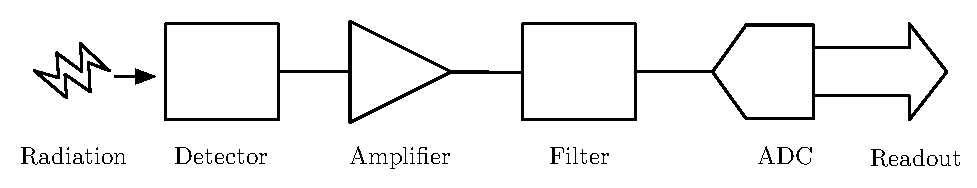
\includegraphics[width=5in]{./Figures/detector.eps}
	\caption{Block diagram for a single channel, generic instrumentation circuit for particle physics experiments.}
	\label{fig:intint}
\end{figure}

The initial amplifier translates the input charge signal, coming from the detector electrodes, into an output voltage signal. Charge-to-voltage translation is done by transferring the charge $Q_{in}$ from the nonlinear detector capacitance to a linear, known capacitor $C$. The generated voltage $V_{out}$ is simply given by $V_{out} = Q_{in}/C$, with $C$ easily and precisely tailorable. Fig.~\ref{fig:csa_post} depicts the most common preamplifier implementation, which consists of a voltage amplifier with a capacitor in a negative feedback configuration. The resulting feedback circuit is a charge-sensitive amplifier (CSA), extensively studied in the literature \citep{Snoeys100,Asp100,deGeronimo500,oconnor100,Alvarez101}. The amplified detector signal includes noise from the detector and the amplifier. Since the noise statistics are well modeled, they can be used to design a filter that maximizes the signal-to-noise ratio (SNR) at the detector front-end. Usually the filter is an analog block, either time-invariant or time-varying, used to convert the voltage signal at the CSA output into a shaped voltage pulse. The pulse shape defines the weights of noise sources on the front-end output noise. Thus, a proper selection of the pulse shape is part of the solution to the SNR maximization problem. A memory acts as a buffer necessary to store data for a number of events before readout. For high-frequency pulse trains, analog memory is particularly well suited \citep{Kleinfelder100,Haller100}. Filtered signals can be quickly stored as charge in integrated capacitors, to be converted into digital signals by dedicated ADCs during the readout phase. Integration and feature size reduction has allowed the design of highly dense digital memory arrays. If a digital memory is used instead, ADCs are used to digitize the signal prior to storage, and conversion throughput per IC must be as high as the collision rate times the number of channels. 

\begin{figure}[!t]
	\centering
	\includegraphics[width=2in]{./Figures/csa_post}
	\caption{CSA using a voltage amplifier. Detector is modeled as a photodiode.}\label{fig:csa_post}
\end{figure}


\section{Noise minimization in circuits for particle physics instrumentation}
\subsection{Basic notions}
In electronics, noise is a random fluctuation in an electrical signal, and is present in all electronic circuits. It constitutes an important issue in the design of integrated circuits, since it affects the accuracy of the signals processed. Noise generated by electronic devices, such as bipolar transistors and MOSFETs, varies greatly, as it can be produced by several different physical processes. There are three sources of fundamental noise in MOSFETs \citep{gray101}: shot noise due to gate leakage current, thermal (for strong inversion operation) or shot (for weak inversion operation) noise in the channel, which is always white, and flicker or $1/f$ noise, also called low-frequency noise. These noise sources have been widely studied throughout the years, and several works about them can be found in the literature. References \citep{gray101,jindal101} are good starting points for introducing the reader into this subject.

Noise is naturally expressed as a frequency-dependent power spectral density, in either $V^2/\textit{Hz}$ or $A^2/\textit{Hz}$. The integral of the noise power spectrum over the circuit bandwidth yields the total circuit noise power, and its square root is the standard deviation of either the noise voltage or noise current.

In an electronic circuit, composed by a number of electronic devices, there are several noise sources. To quantify the effect of these different noise sources, each one of them can be referred to a common node of the circuit, typically the input node. Noise sources referred to the same node are added as power as follows 
\begin{equation}
\sigma^2_\textit{Total} = \sigma^2_1 + \sigma^2_2 + 2\cdot c \cdot \sigma_1 \cdot \sigma_2
\end{equation}
where $\sigma_i^2$ represents the noise power of source $i$, and $c$ is the correlation coefficient between the two noise sources. If both noises come from the same physical process (i.e., they are fully correlated), $c = 1$ and $\sigma_\textit{Total} = \sigma_1 + \sigma_2$ is given by the sum of the noise signals; if the noises come from different noise sources, they are usually not correlated ($c = 0$) and $\sigma^2_\textit{Total} = \sigma^2_1 + \sigma^2_2$ is the given by the sum of individual powers.

By referring the noise sources to the input of the system, it is possible to make a fair comparison of noise performance among different systems with different gains, and set the total input-referred noise as a figure of merit. In a linear circuit, the total input- referred noise can be represented by a combination of a series voltage noise source ($V_n^2$) and a parallel current noise source ($I_n^2$), as shown in Fig.~\ref{fig:noise_cir}. If the driving signal is a low-impedance voltage source, only the voltage noise is important, whereas if the signal source is a high-impedance current source, the voltage noise can be neglected, as current noise accounts for all the system noise. In system with a non-ideal load line, both noise sources must be considered.

\begin{figure}[!t]
	\centering
	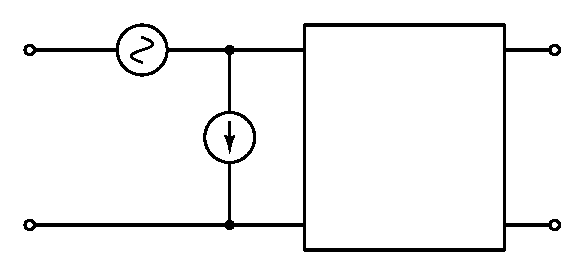
\includegraphics[width=3.2in]{./Figures/noise_cir}
	\caption{Equivalent representation of a linear circuit internal noise sources referred to the input port.}\label{fig:noise_cir}
\end{figure}

\subsection{Current trends in noise minimization for particle physics instrumentation systems}
Noise minimization in particle physics experiments is done by a careful design of the channel, and specifically, on the detector, CSA and filter parameters. Understanding and designing for low noise has been one of the main concerns in modern particle physics instrumentation. Any survey on this topic starts with a work published in 1968 \citep{radeka104}, where important concepts of pulse shaping for particle physics experiments were described. At this time, the search for practical optimum shapers and simpler analysis methods were the main concerns. The concept of a weighting function, equivalent to impulse response, but valid for time-varying systems as well, was introduced.

In 1972, a powerful time-domain analysis technique was published \citep{goulding101}, for comparing the filtering effects of different pulse shapers. Starting from a physical approach and assuming only white noise, it was shown that all the noise sources in a front-end for particle physics experiments can be reduced to two components at the input node: step (parallel) noise and delta (series) noise. Integration of each component in frequency yields two noise coefficients that make it possible to characterize the noise-filtering capabilities of a pulse shaper, independently of the time scale. These ideas are still in use today.

In 1984, a good review and some examples of readout electronics techniques for semiconductor detectors in particle physics instrumentation systems was published \citep{gatti103}. The author emphasized the importance of the input stage of the front-end electronics in the overall noise performance. By that time, there was already some interest in MOS technology (with lower performance than JFETs or MESFETs) due to the potential of integrating the semiconductor detector and its electronics. In the same year, a good summary of semiconductor position-sensitive detectors was also published \citep{radeka105}. It was shown that the minimum noise is achieved when the detector and amplifier input capacitances are matched.

In 1988, one of the most influential papers in low-noise techniques for particle physics instrumentation was published \citep{radeka101}. In this paper, the results from previous works on noise were summarized.

Flicker noise research in particle physics electronics was published in 1989 \citep{lutz101}. Before this paper, flicker noise was rarely mentioned and seldom considered in analysis equations for particle physics electronics. In 1990, the issue of optimum shapers for particle physics electronics, including low frequency noise in the analysis, was published \citep{gatti104}. The same year, an excellent derivation of noise for particle physics front-end electronics, including thermal, flicker and shot noise sources was presented \citep{sansen101}.

In 1992 \citep{gadomski101}, the deconvolution method for pulse-shaping was presented. Major innovations of this work come from the use of switched-capacitor filters for \mbox{pulse-processing} purposes and the introduction of the concept of \mbox{discrete-time} \mbox{pulse-shaping}.

In 1998 \citep{pullia104}, for the first time the contribution of the low-frequency noise is computed in the time domain, using fractional derivatives. It is an extension of earlier noise computation methods \citep{goulding101}. A generalization of this work was presented in 2004 \citep{pullia102}, allowing time-domain simulations of almost all kind of noise sources.  This work represents a powerful tool for computer-aided filter design.


%In 2001, a nice overview of front-end electronics for imaging detectors, oriented to particle physics applications was published [7]. In that work, neat and simple equations to compute the equivalent noise charge from white, flicker and shot sources were presented. The same equations are employed in a later publication [12], where it is shown that, using more accurate transistor and noise models, minimum noise is not necessarily achieved when maximum available power and capacitance matching conditions are fulfilled. 
%It is also shown that the low frequency noise contribution may depend on the shaper time constant, a result not found before using simpler equations.

Finally, excellent books on particle physics instrumentation systems have been published \citep{radeka201}, compiling and explaining the results from many papers in the field.


\section{Thesis content}
Chapter 2 starts with an introduction to the project that prompts the work of this thesis, the design and implementation of a second iteration of The Bean, an instrumentation application-specific integrated circuit (ASIC) which forms part of the proposal for the ILC. It is followed by an overview of the motivations that led to the development of a new mathematical framework for noise analysis in discrete-time filters, alongside with the presentation of the requirements for a filter intended to take full advantage of this framework. Chapter 3 presents the complete formulation of this noise analysis, including examples and applications for optimal filter computation. In Chapter 4 , the design and implementation of a filter for arbitrary weighting function synthesis are presented. Chapter 5 shows the results that contribute to the ongoing project, functionality verifications of the designed filter and the implementation of an early prototype of The Bean 2, with the filter as one of its core building blocks. Finally, Chapter 6 summarizes the results and contributions of this work, and presents ideas for future research.